\documentclass{oci}
\usepackage[utf8]{inputenc}
\usepackage{amssymb}
\usepackage{tikz}

\newcommand{\drawarr}{
    \draw[thick] (0,0) grid (4,-1);

	\node at (0.5,-1.3) {\small 0};
	\node at (1.5,-1.3) {\small 1};
	\node at (2.5,-1.3) {\small 2};
	\node at (3.5,-1.3) {\small 3};

    \node at (0.5,-0.5) {1};
    \node at (1.5,-0.5) {-1};
    \node at (2.5,-0.5) {1};
    \node at (3.5,-0.5) {1};
}

\newcommand{\drawlayerl}[1]{
\pgfmathsetmacro{\b}{#1 - 0.02}
\fill[white,opacity=0.8] (-0.1,0.1) rectangle (\b,-1.5);
}
\newcommand{\drawlayerr}[1]{
\pgfmathsetmacro{\a}{4.02 - #1}
\fill[white,opacity=0.8] (\a,0.1) rectangle (4.02,-1.5);
}

\newcommand{\drawsubarr}[2]{
	\drawarr{}
	\drawlayerl{#1}
	\drawlayerr{#2}
}

\newcommand{\yes}{
	\node at (4.8, -0.5) {\LARGE $\checkmark$};
}
\newcommand{\crossmark}{$\mathbin{\tikz [x=1.4ex,y=1.4ex,line width=.2ex] \draw (0,0) -- (1,1) (0,1) -- (1,0);}$}%

\newcommand{\no}{
	\node at (4.8, -0.5) {\LARGE \crossmark{}};
}



\title{Apuesta}

\begin{document}
\begin{problemDescription}
Fernanda y decidió hacer una apuesta de alto riesgo con sus amigos.
Fernanda lanza una moneda.
%
Si cae cara, pasarán a la Industria Chilena de Papas Caseras (ICPC)
a comerse una porción de papas, de lo contario, se quedarán de brazos cruzados todo el día.
%
Lamentablemente, la moneda cayó sello, por lo que el destino decidió que se perderían
de esta increíble oportunidad.
%
Pero Fernanda, no contenta con el resultado, decidió hacer una nueva apuesta en la que
está segura podrá ganar.

En esta nueva apuesta, Fernanda lanza $n$ monedas
y anota los resultados en una lista.
%
Podemos representar esta lista con un arreglo de
enteros dónde 1 representa que la moneda cayó
cara y -1 que cayó sello.
%
La siguiente figura representa un escenario
con 4 monedas.
%
\begin{center}
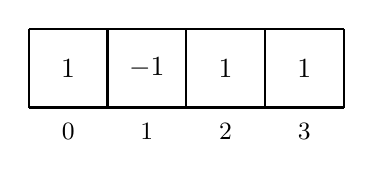
\begin{tikzpicture}
\draw[thick] (0,-1) grid (4,0);
\node at (0.5,-1.3) {\small 0};
\node at (1.5,-1.3) {\small 1};
\node at (2.5,-1.3) {\small 2};
\node at (3.5,-1.3) {\small 3};
\node at (0.5,-0.5) {$1$};
\node at (1.5,-0.5) {$-1$};
\node at (2.5,-0.5) {$1$};
\node at (3.5,-0.5) {$1$};
\end{tikzpicture}
\end{center}
Para ganar la apuesta, Fernanda debe contar la cantidad de subarreglos
contiguos donde la cantidad de caras es estrictamente mayor
que la cantidad de sellos.
%
Si un subarreglo cumple con esta condición decimos que el subarreglo
es exitoso.
%
Si el número de subarreglos exitosos es la mayoría, entonces
Fernanda ganará la apuesta y cumplirá su sueño de ir a la ICPC.

La siguiente figura muestra todos los subarreglos para el ejemplo
anterior.
%
Cada caso está marcado con un ticket ($\checkmark$)
si el subarreglo es exitoso o con una cruz (\crossmark{}) si no lo es.
%
En este caso, como la cantidad subarreglos exitosos es la mayoría,
Fernanda ganaría la apuesta.

\begin{minipage}{0.48\textwidth}
	\begin{center}
		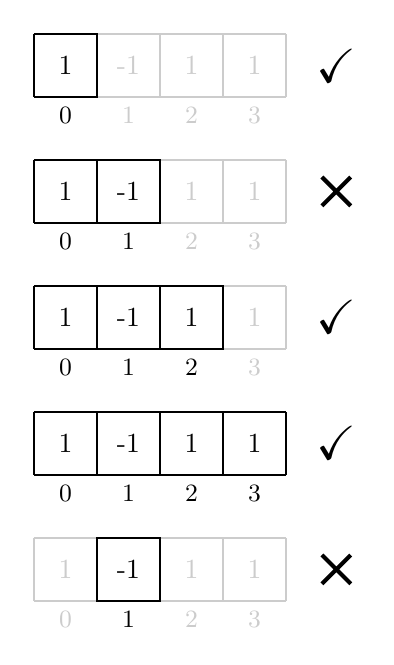
\begin{tikzpicture}[scale=0.8]
			\begin{scope}[yshift=0cm]
			\drawsubarr{0}{3};
			\yes{};
			\end{scope}

			\begin{scope}[yshift=-2cm]
			\drawsubarr{0}{2};
			\no{}
			\end{scope}

			\begin{scope}[yshift=-4cm]
			\drawsubarr{0}{1};
			\yes{}
			\end{scope}

			\begin{scope}[yshift=-6cm]
			\drawsubarr{0}{0};
			\yes{}
			\end{scope}

			\begin{scope}[yshift=-8cm]
			\drawsubarr{1}{2};
			\no{}
			\end{scope}
		\end{tikzpicture}
	\end{center}
\end{minipage}
\begin{minipage}{0.48\textwidth}
	\begin{center}
		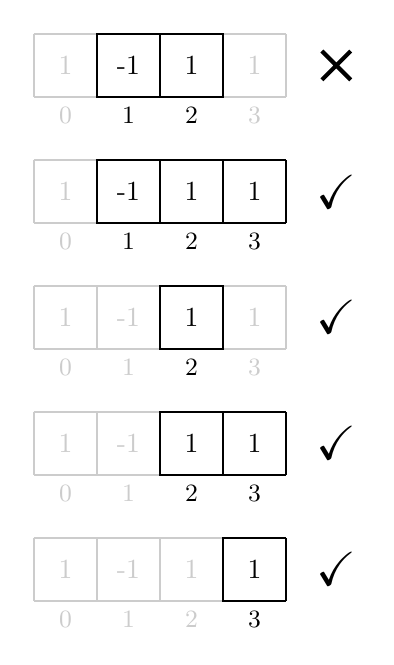
\begin{tikzpicture}[scale=0.8]
			\begin{scope}[yshift=0cm]
			\drawsubarr{1}{1};
			\no{}
			\end{scope}

			\begin{scope}[yshift=-2cm]
			\drawsubarr{1}{0};
			\yes{}
			\end{scope}

			\begin{scope}[yshift=-4cm]
			\drawsubarr{2}{1};
			\yes{}
			\end{scope}

			\begin{scope}[yshift=-6cm]
			\drawsubarr{2}{0};
			\yes{}
			\end{scope}

			\begin{scope}[yshift=-8cm]
			\drawsubarr{3}{0};
			\yes{}
			\end{scope}
		\end{tikzpicture}
	\end{center}
\end{minipage}

Fernanda ya lanzó las monedas y se puso a contar la cantidad de subarreglos
exitosos.
% exitosos y totales utilizando sus conocimentos avanzados de combinatoria.
A pesar de sus avanzados conocimientos de combinatoria, se está demorando mucho
y la ICPC cierra en menos de 4 horas.
%
?`Podrías ayudarla a contar la cantidad de subarreglos exitosos para
que alcance a ir a la ICPC antes de que cierre?
\end{problemDescription}

\begin{inputDescription}
La primera línea contiene un único entero $n$ $(1 \leq n \leq 10^6)$, correspondiente
a la cantidad de monedas.

La segunda línea contiene $n$ enteros.
%
El entero $i$-ésimo corresponde al resultado de lanzar la $i$-ésima moneda.
%
El valor será 1 si la moneda cayó cara y -1 si cayó sello.
\end{inputDescription}

\begin{outputDescription}
La salida debe contener un único entero correspondiente a la cantidad
de subarreglos exitosos, es decir, la cantidad de subarreglos donde
la cantidad de caras es estrictamente mayor que la cantidad de sellos.
\end{outputDescription}

\begin{scoreDescription}
	\subtask{10} Se probarán varios casos de prueba donde $n \leq 4$.
	\subtask{20} Se probarán varios casos de prueba donde $n \leq 100$.
  	\subtask{30} Se probarán varios casos de prueba donde $n \leq 10^4$.
	\subtask{40} Se probarán varios casos de prueba sin restricciones adicionales.
\end{scoreDescription}

\begin{sampleDescription}
\sampleIO{sample-1}
\sampleIO{sample-2}
\end{sampleDescription}

\end{document}
